

\chapter{Mask R-CNN}

\section{Fonctionnement d'un Mask R-CNN}

\subsection{Introduction}

La première partie de ce nouveau projet consistait à détecter toutes les formes humaines présentes sur une image. Malheureusement, une simple structure de CNN ne suffit pas pour effectuer cette tâche. En effet, plusieurs difficultés gênent son bon fonctionnement : l'image n'est pas forcément cadrée pour contenir exactement l'objet que le CNN est sensé détecter, celui-ci ne donne aucune indication quant à la position de cet objet dans l'image ni même ses contours. Une nouvelle architecture a donc dû être utilisée: les \textbf{Mask R-CNN}. La figure \ref{result_mask_r_cnn} montre ce que l'on peut obtenir avec une telle architecture.

\begin{figure}[!h]
\centering
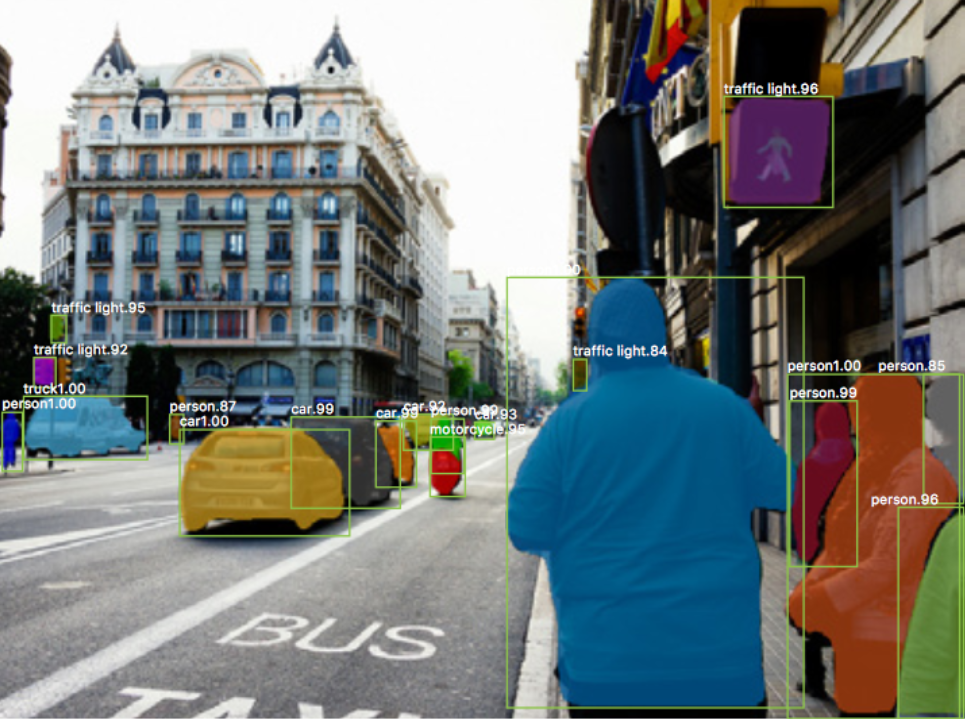
\includegraphics[width=200pts]{images/Mask_R_CNN/mask_r_cnn.png} 
\caption{Exemple de résultats obtenus avec un Mask R-CNN}
\label{result_mask_r_cnn}
\end{figure}

\subsection{Présentation générale}

Les Mask R-CNN ont fait leur apparition en 2017, sous l'impulsion d'une équipe de chercheurs de Facebook. La technique s'est rapidement démocratisée pour aujourd'hui devenir un incontournable de la segmentation d'images. Le principe directeur est le suivant :
 \begin{itemize}
\item Extraction des caractéristiques sémantiques de l'image
\item Traitement pour gérer la taille des objets : FPN (Feature Pyramid Network)
\item Proposition de régions contenant des objets :RPN (Region Proposal Network)
\item Redimensionnement des régions : ROI Align
\item Réseau donnant la classe d'objets de chaque région et leur redimensionnement
\item Suppression des régions redondantes : Non Max Suppression
\item Réseau donnant les masques
\end{itemize}

A titre d'information, la figure \ref{R_CNN_structure} résume sommairement la structure d'un Faster-R-CNN, à laquelle nous allons nous intéresser par la suite.

\begin{figure}[!h]
\centering
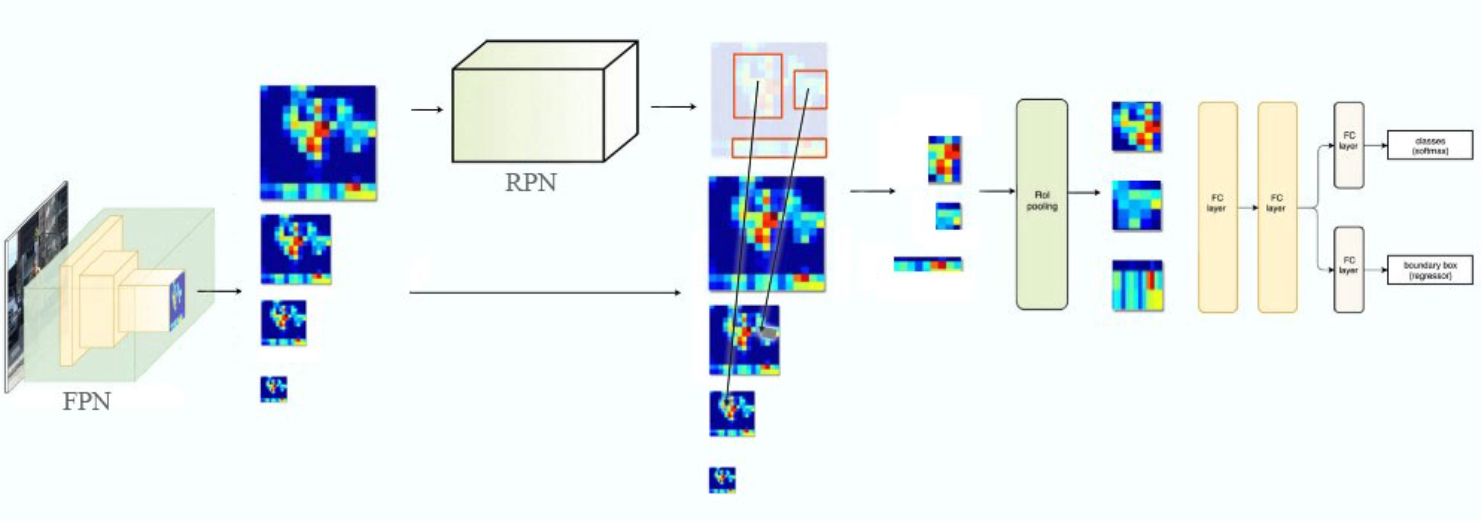
\includegraphics[width=300pts]{images/Mask_R_CNN/R_CNN_structure.png} 
\caption{Structure d'un R-CNN}
\label{R_CNN_structure}
\end{figure}



\subsection{Extraction des caractéristiques sémantiques de l'image}

Les Mask R-CNN reposent sur une structure de Faster R-CNN, architecture qui permet de donner les boîtes englobantes (bounding box) ainsi que la classe de l'objet compris dedans. Celle-ci est plus rapide (faster) qu'un R-CNN basique dans la mesure où elle ne procède qu'une seule fois à l'extraction des caractéristiques. Ainsi, on fait passer l'image d'entrée par un réseau à couches de convolutions tel que ResNet et on extrait les dernières afin d'avoir une carte des caractéristiques de l'image, nous donnant in fine une compréhension sémantique de celle-ci.

\begin{figure}[!h]
\centering
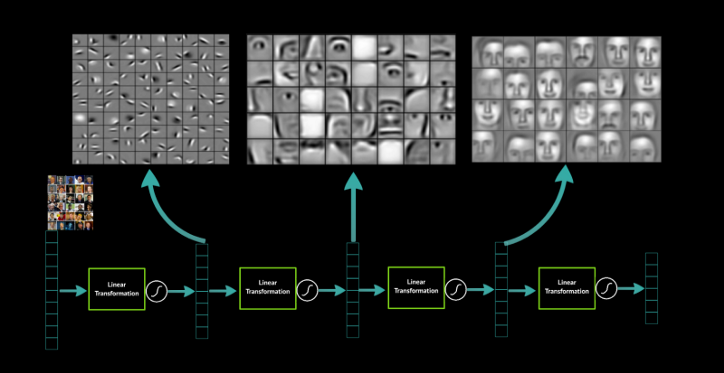
\includegraphics[width=200pt]{images/Mask_R_CNN/resnet_extraction.png} 
\caption{exemple d'extraction de motifs, on garderait ici les dernières couches.}
\label{resnet_extraction}
\end{figure}

\subsection{Region Proposal Network}

L'étape suivante consiste à proposer des régions d'intérêt (ROI : Region of Interest) afin de déceler au mieux les objets présents sur l'image. Pour cela, l'algorithme se base sur des formes prédéfinies, les \textbf{anchors}. En effet, il est raisonnable de supposer que les objets que nous cherchons à détecter ont globalement tous des boîtes englobantes qui sont des formes suivantes : carrés plus ou moins grands, rectangles horizontaux ou verticaux eux aussi plus ou moins grands. Il faut bien comprendre ici que l'hypothèse se fait sur le ratio de ces boîtes (par exemple au pire 1 pour 3). Un exemple est montré sur la figure \ref{anchors}.

\begin{figure}[!h]
\centering
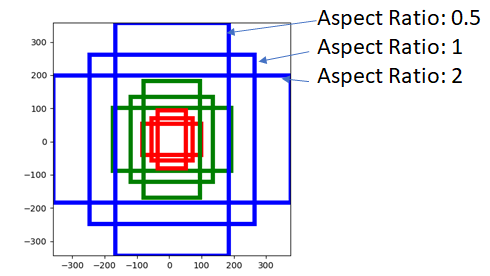
\includegraphics[width=200pt]{images/Mask_R_CNN/anchors.png} 
\caption{exemple d'un ensemble d'anchors}
\label{anchors}
\end{figure}

A partir de cette ensemble défini arbitrairement, il suffit de faire un quadrillage sur l'image, et pour chacun des points, proposer comme région chacune des anchors centrées en ce même point. Un exemple de cette technique est montrée figure \ref{proposed_anchors}.

\begin{figure}[!h]
\centering
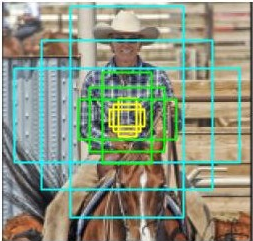
\includegraphics[width=150pts]{images/Mask_R_CNN/proposed_anchors.png} 
\caption{exemple d'un sous ensemble de régions proposées par le RPN : on ne montre ici que les régions centrées en un point par soucis de lisibilité, mais il faut bien comprendre que ce processus est itéré sur tous les points de la grille}
\label{proposed_anchors}
\end{figure}

\subsection{Feature Pyramid Network}

L'un des grand avantages du Mask R-CNN repose dans la structure de Feature Pyramid Network (FPN). Tout part de la constatation que la détection des objets se fait beaucoup plus facilement avec des cartes de caractéristiques dont la compréhension sémantique est grande. Malheureusement, celles-ci sont de petites tailles, ce qui pose problème pour le bon placement des régions d'intérêt, car plus l'image est comprimée, plus on perd d'informations sur la disposition précise des objets sur l'image non compressée. L'astuce a alors été de créer une structure pyramidale, où chaque étage correspond à une carte des caractéristiques (extraite dans le ResNet), de plus en plus petite au fur et à mesure que le numéro de l'étage augmente. Le principe est illustré sur la figure \ref{FPN_1}.

\begin{figure}[!h]
\centering
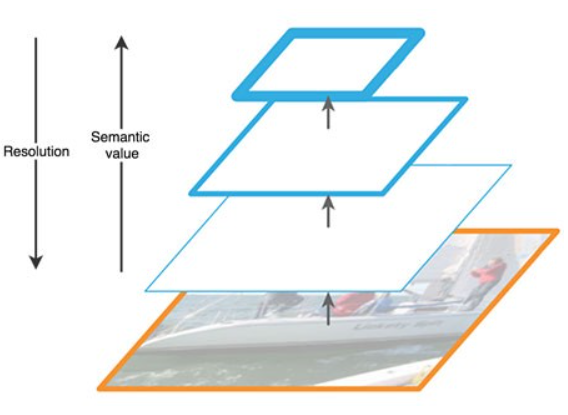
\includegraphics[width=200pts]{images/Mask_R_CNN/FPN_1.png} 
\caption{Structure de la pyramide : à noter l'incompatibilité entre la compréhension sémantique et la résolution}
\label{FPN_1}
\end{figure}

Ensuite, l'algorithme essaye de prédire si la région d'intérêt considérée comprend oui ou non un objet. Pour cela, il essaye de redescendre cette pyramide afin d'avoir plusieurs niveaux de compréhension. La figure \ref{FPN_2} explique le principe.

\begin{figure}[!h]
\centering
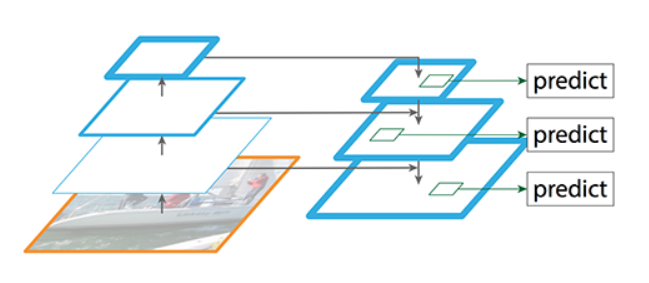
\includegraphics[width=200pts]{images/Mask_R_CNN/FPN_2.png} 
\caption{Top-Down pathway : chaque étage est le résultat de la somme éléments par éléments du grossissement par 2 de l'étage supérieur (par interpolation) et de la carte de caractéristiques correspondante auquel on a appliqué une convolution 1 $\times$ 1 (dans le but de réduire à 1 la profondeur de celle-ci). L'étage supérieur est simplement construit avec un étage supérieur fictif égal à la matrice 0. Remarquons que chaque étage est relié à sa carte correspondante afin de régler au mieux le positionnement de la région d'intérêt.}
\label{FPN_2}
\end{figure}

Chaque étage essaye alors de prédire si oui ou non la région d'intérêt correspondante contient un objet ou non. Enfin, pour savoir à quel étage se fier, on se rapporte à la dimension de la région, en appliquant la formule suivante :

$$k = \lfloor k_0 + log_2( \frac{ \sqrt{wh}}{224} ) \rfloor $$

où :\\
$k_0 = 4$\\
w : largeur de la région\\
h : hauteur de la région\\

Il suffit alors de prendre l'étage k, où l'étage 0 correspond à celui de plus grande taille. On comprend donc intuitivement que plus la région est grande, plus l'éventuel objet associé est grand, plus on peut se permettre d'aller dans les détails, et donc de monter dans les étages de la pyramide. Au contraire, plus la région est petite, plus celle-ci va se perdre dans les rétrécissements successifs, et il est donc plus raisonnable de rester dans les couches larges bien que cela soit pénalisant en termes de sémantique.\\
\\
Une fois cette étape passée, il suffit de garder la région d'intérêt si et seulement si le réseau considère qu'elle contient un objet.

\subsection{Phase de Pooling}

Ensuite, à partir des régions d'intérêt proposées par le RPN, il faut pouvoir extraire la partie de l'image correspondante sur la carte des caractéristiques choisie, ce qui pose problème dans la mesure où celle-ci est plus petite que l'image originelle. Pour cela, une première technique naïve a été mise en oeuvre : Le \textbf{ROI pooling}. 

\subsubsection{ROI Pooling}

Cette méthode consiste à diviser les dimensions de la région d'intérêt  et sa position par le nombre de fois que la carte des caractéristiques   a été réduite par rapport à l'image originelle. Par exemple, si la carte est au niveau 2 de la pyramide de la méthode FPN, elle est 4 fois plus petite que l'image, et donc on réduit par 4 la région d'intérêt. Malheureusement, les grandeurs résultantes ne sont pas forcément entières, ce qui force la méthode à prendre la partie entière du résultat. Un exemple de fonctionnement est montré figure \ref{ROI_Pooling}.

\begin{figure}[!h]
\centering
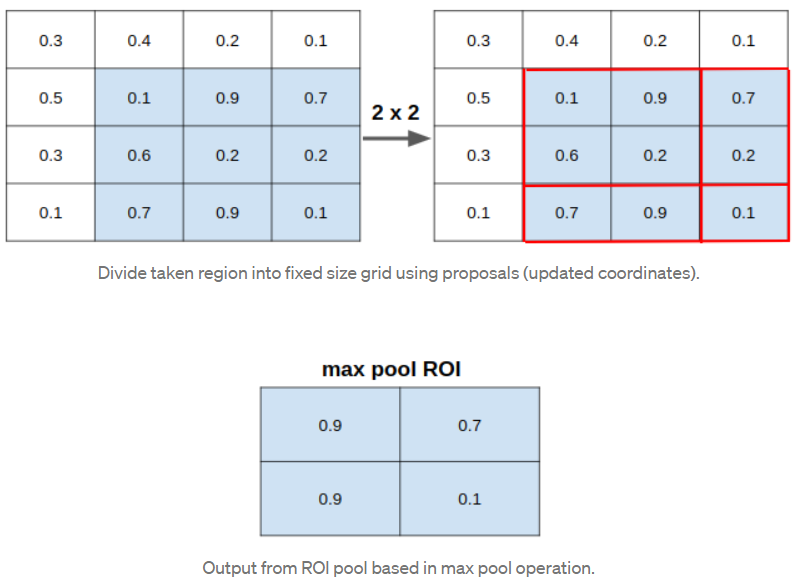
\includegraphics[width=200pts]{images/Mask_R_CNN/ROI_Pooling.png} 
\caption{Fonctionnement du ROI Pooling : on part d'une région $3 \times 3$ que l'on veut réduire à une région $2 \times 2$. Lors de la division avec partie entière, on se rend compte qu'un décalage se forme pour la position, ce qui pousse la partie supérieure gauche de la nouvelle région à représenter plusieurs valeurs. On applique donc un max pooling (on garde le maximum de chaque zone) et le résultat final est obtenu.}
\label{ROI_Pooling}
\end{figure}

Cependant, les chercheurs se sont rendus compte que cela posait un problème. En effet, même si la classification est quasi insensible au décalage créé par la partie entière, la pratique a révélé que la position et forme des masques étaient beaucoup moins précises. La figure \ref{ROI_pooling_problem} illustre ce phénomène sur un exemple simple.

\begin{figure}[!h]
\centering
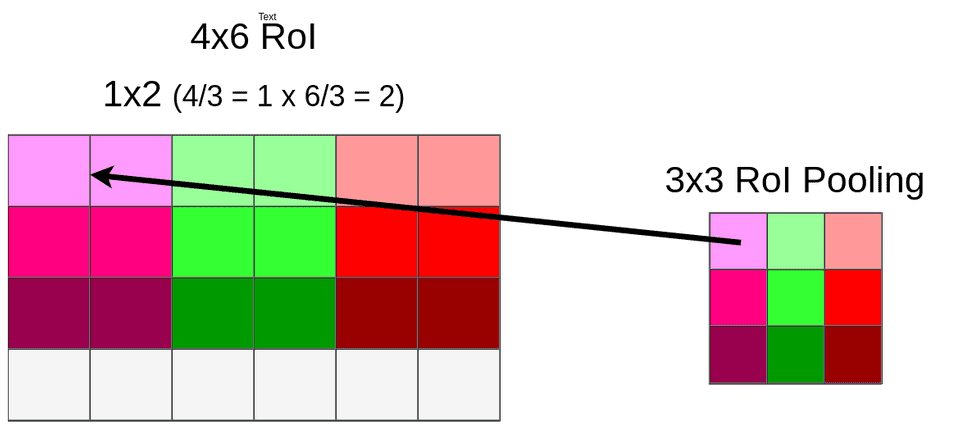
\includegraphics[width=200pts]{images/Mask_R_CNN/ROI_pooling_problem.png} 
\caption{Problème de reconstruction de masques avec le ROI Pooling : une fois que l'on a une région qui possède un objet bien classifié avec un masque (dont on verra plus tard qu'il est lui aussi initialement construit à des échelles inférieures à l'image originelle), il faut à nouveau pouvoir l'agrandir pour avoir un masque à l'échelle. Or il est possible de voir sur cet exemple que le redimensionnement de celui-ci créé des duplications, décalages et déformations sur le résultat final, en témoignent les parties gauches et droites de la région initiale qui sont étirées sur le résultat final}
\label{ROI_pooling_problem}
\end{figure}

Une nouvelle méthode est alors naturellement apparue pour contrer ce phénomène : le \textbf{ROI Align}.

\subsubsection{ROI Align}

la méthode ROI Align fonctionne de la même manière que ROI Pooling à l'exception que celle-ci garde les valeurs réelles des nouvelles positions, ce qui la pousse à procéder à un traitement supplémentaire pour prendre en compte les parties fractionnaires.\\
En effet, une cellule du résultat final va ici représenter les différentes cellules qu'elle est sensée représenter par une méthode d'interpolation bilinéaire. La figure \ref{ROI_Align} explique graphiquement ce mécanisme.

\begin{figure}[!h]
\centering
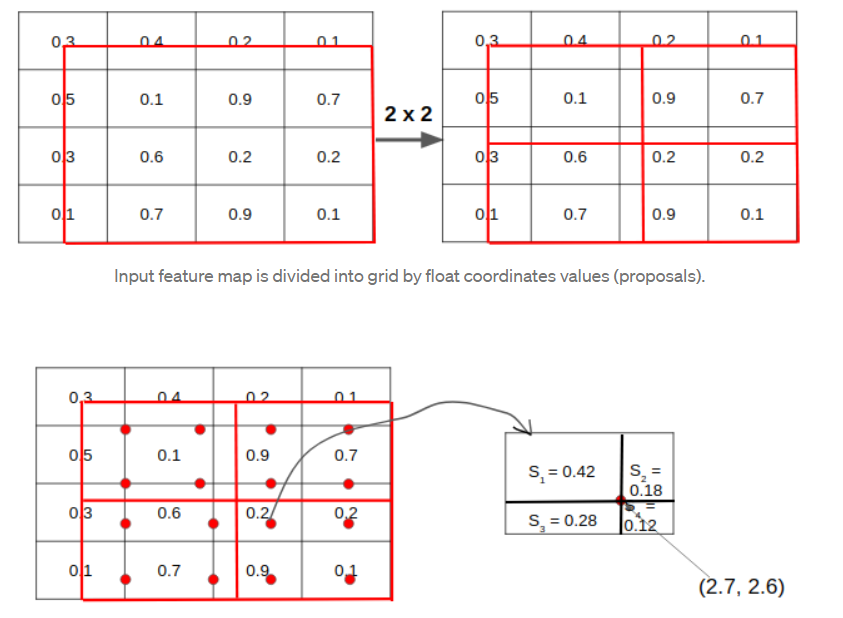
\includegraphics[width=200pts]{images/Mask_R_CNN/ROI_Align.png} 
\caption{Fonctionnement du ROI Align : on place la région à sa position en valeurs réelles, on la découpe en le nombre voulu de cellules, on place 4 points pour chacune de ces cellules afin de procéder à l'interpolation bilinéaire. Il suffit alors d'effectuer un max pooling pour obtenir le résultat final.}
\label{ROI_Align}
\end{figure}

Ainsi, grâce à cette méthode, les problèmes liés à la division en partie entière disparaissent, et on observe bien en pratique des rendus bien meilleurs pour les masques avec le ROI Align comparativement au ROI Pooling.

\subsection{Classification et réglage des boites englobantes}

Une fois que l'on a toutes les régions d'intérêt avec pour chacune d'elles la partie de la carte des caractéristiques correspondante, il suffit de les faire passer par un réseau dense (fully connected layers) afin de prédire et la classe de l'objet contenu dans la région, et pour chacune des classes les ajustements à produire sur cette région afin d'obtenir la boite englobante la plus pertinente. Par exemple, si on a K classes, la sortie sera de dimension K+1 (en comptant l'objet background) + 4 * K (où le 4 correspond au nombre de données d'ajustement de la boîte). De plus, on se doute bien que les anchors n'ont pas parfaitement la forme adéquate, et le réseau s'occupe lui-même de trouver numériquement comment modifier cette région. \\
\\
Soit \\
$p_x$ : coordonnée x du centre de la région \\
$p_y$ : coordonnée y du centre de la région \\
$p_w$ : largeur de la région \\
$p_h$ : hauteur de la région \\

Algorithmiquement, le réseau cherche les valeurs $d_x,d_y,d_w,d_h$ telles que :\\
\\
$\hat{p_x} = p_w d_x + p_x$\\
$\hat{p_y} = p_h d_y + p_y$\\
$\hat{p_w} = p_w e^{d_w}$ \\
$\hat{p_h} = p_h e^{d_h}$\\

La figure \ref{redimensionnement} exprime graphiquement le but de ce réseau.

\begin{figure}[!h]
\centering
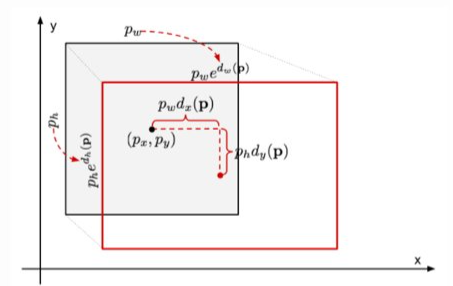
\includegraphics[width=200pts]{images/Mask_R_CNN/redimensionnement.png} 
\caption{illustration graphique de l'objectif de recadrage et redimensionnement du réseau}
\label{redimensionnement}
\end{figure}

Explicitons à présent la fonction de coût d'un tel réseau. Pour cela, nous allons introduire quelques valeurs utiles :\\
\\
$N_{classes}$ : nombre de classes \\
$N_{boxes}$ : nombre de boites englobantes \\
$\hat{p}^c_i$ : probabilité prédite que la boite i soit de classe c \\ 
$p^c_i$ : probabilité réelle que la boite i soit de classe c (ground truth) \\ 
$\hat{t}^c_i$ : vecteur $4 \times 1$ des coordonnées de la boite englobante prédite \\ 
$t^c_i$ : vecteur $4 \times 1$ des coordonnées de la boite englobante réelle (ground truth) \\
$\lambda$ : un paramètre d'ajustement\\
\\
La fonction de coût du réseau peut maintenant être explicitée :
$$\mathcal{L}_{tot} = \mathcal{L}_{classes} + \mathcal{L}_{boxes}$$ 
$$= \frac{1}{N_{classes}} \sum_{i,c} \mathcal{L}_{classe}(p^c_i,\hat{p}^c_i) + \frac{ \lambda}{N_{boxes}} \sum_{i,c} p^c_i \times \mathcal{L}^1_{smooth}(t^c_i - \hat{t}^c_i)$$\\
\\
Où $\mathcal{L}_{classe}$ correspond à une cross-entropie classique.\\
\\
On remarque que cette fonction de coût est divisée en deux parties : la première s'occupe de gérer la bonne classification de l'objet dans la boite i, et la deuxième gère les boites englobantes, en vérifiant que celle qui importe (d'où la multiplication par $p_i$) correspond bien à la boite englobante que l'on veut. A noter également que la fonction $\mathcal{L}^1_{smooth}$ a un comportement un peu différent de la fonction $\mathcal{L}^1$ comme le montre son tracé figure \ref{L1_smooth}.

\begin{figure}[!h]
\centering
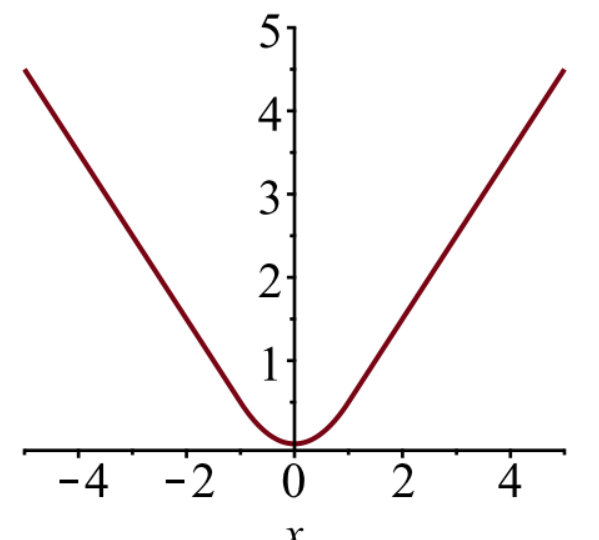
\includegraphics[width=100pts]{images/Mask_R_CNN/L1_smooth.png} 
\caption{tracé de la fonction $\mathcal{L}^1_{smooth}$}
\label{L1_smooth}
\end{figure}

\subsection{Non Max Suppression}

Cependant, si nous utilisions l'algorithme directement, on n'aurait pas le résultat attendu. En effet, nous aurions beaucoup trop de boites englobantes pour un même objet. Actuellement, rien n'oblige un objet a avoir une multitude de boites englobantes. La méthode \textbf{Non Max Suppression} s'attelle à corriger ce problème en éliminant toutes les boites redondantes. Pour cela elle se base sur une métrique classique en traitement d'image : l'\textbf{IoU} (Intersection over Union). Celle-ci mesure simplement à quel point deux rectangles sont proches d'un point de vue spatial l'un de l'autre. La figure \ref{IoU} exprime graphiquement le calcul de cette métrique.

\begin{figure}[!h]
\centering
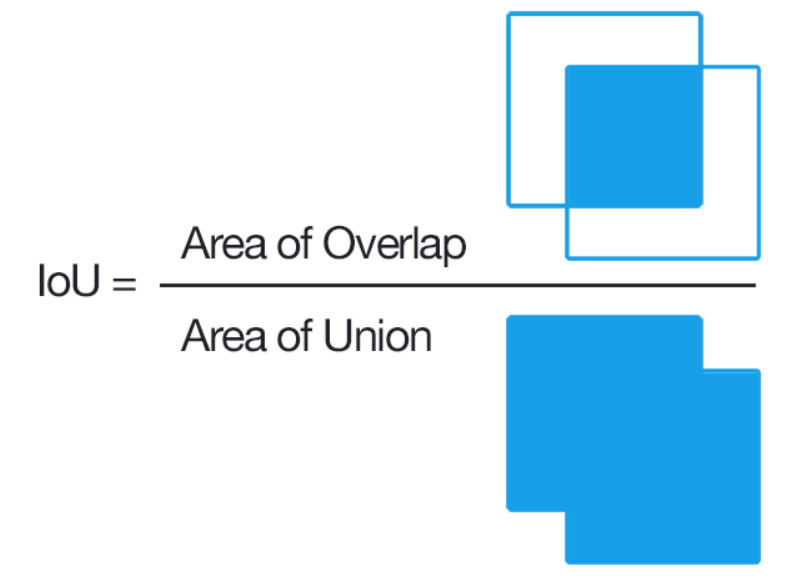
\includegraphics[width=100pts]{images/Mask_R_CNN/IoU.png} 
\caption{calcul de la métrique IoU : il suffit de faire le rapport entre l'aire de l'intersection entre les deux rectangles et l'aire de l'union de ces deux rectangles.}
\label{IoU}
\end{figure}

Ainsi, on comprend que plus la métrique est proche de 1, plus les deux boites sont similaires. La méthode \textbf{Non Max Suppression} exploite ce principe. Premièrement, on choisit la boite englobante avec la plus grande probabilité de contenir un objet. Pour toutes les autres, on calcule l'IoU avec la boite référente et si celui-ci est supérieur à 0.5, on supprime la boite correspondante. Enfin, on répète le processus jusqu'à ce qu'il n'y ait plus de boite avec un IoU supérieur à 0.5 avec une autre boite. La figure \ref{non_max_suppression} montre les résultats d'une telle méthode.

\begin{figure}[!h]
\centering
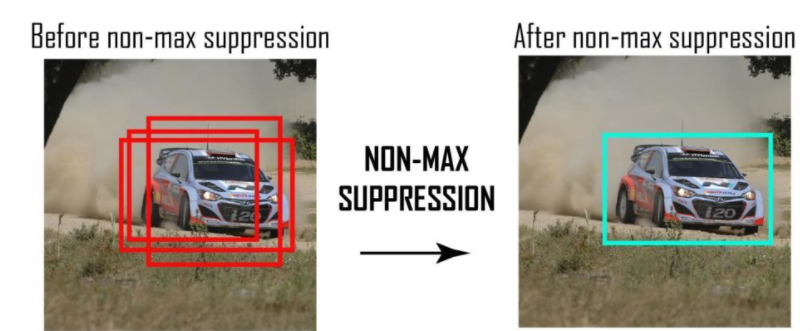
\includegraphics[width=200pts]{images/Mask_R_CNN/non_max_suppression.png} 
\caption{effet de la méthode Non Max Suppression : on observe que toutes les boites englobantes redondantes ont été supprimées au profit de celle qui a la plus grande probabilité de contenir l'objet.}
\label{non_max_suppression}
\end{figure}

\subsection{La gestion des masques}

La gestion des masques a été rajoutée après l'apparition des faster R-CNN, pour donner naissance au Mask R-CNN. La structure globale reste rigoureusement la même, on rajoute juste un réseau de couches de convolutions et déconvolutions supplémentaires à la sortie des cartes de caractéristiques. La figure \ref{Structure_Mask_R_CNN} résume l'architecture d'un Mask R-CNN.

\begin{figure}[!h]
\centering
\includegraphics[width=200pts]{images/Mask_R_CNN/structure_Mask_R_CNN.png} 
\caption{Structure d'un Mask R-CNN}
\label{Structure_Mask_R_CNN}
\end{figure}

Le réseau supplémentaire s'occupe de trouver pour chaque classe un masque $28 \times 28$ qu'il suffit après d'agrandir par déconvolution.
La figure \ref{masks} montre les résultats de ce réseau additionnel.

\begin{figure}[!h]
\centering
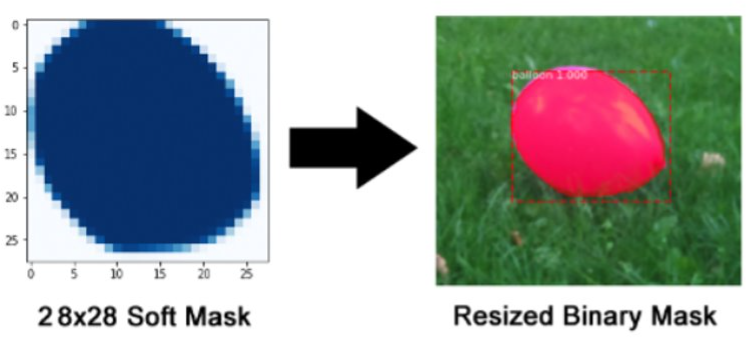
\includegraphics[width=200pts]{images/Mask_R_CNN/masks.png} 
\caption{à gauche : sortie du réseau gérant les masques $28 \times 28$ ; à droite, le masque reconstruit à la bonne échelle}
\label{masks}
\end{figure}

De la même manière, on rajoute à la fonction de coût précédente un nouveau terme gérant l'adéquation des masques avec la réalité :

$$\mathcal{L}_{tot} = \mathcal{L}_{classes} + \mathcal{L}_{boxes} + \mathcal{L}_{masks}$$ 
où 
$$\mathcal{L}_{masks} = -\frac{1}{m^2} \sum_k \sum_{1 \leq i,j \leq m} \hat{p}^k_{i,j}[ \hat{y}^k_{i,j} log(y^k_{i,j} + (1-y^k_{i,j}) log(1-\hat{y}^k_{i,j})]$$

Avec \\
\\
$m = 28$ : taille des masques \\
$y^k_{i,j}$ :supérieur à 0 si le pixel i,j appartient au masque prédit de classe k, 0 sinon \\
$y^k_{i,j}$ : supérieur à 0 si le pixel i,j appartient au masque réel de classe k, 0 sinon (ground truth)\\ 
\\
On remarque que cette fonction de coût ne prend en compte que le masque généré pour l'objet réellement présent dans la boite, et ne considère pas les autres. Ensuite elle se contente de faire une comparaison termes à termes des pixels en passant par une cross-entropie.

\section{Implémentation et Résultats}

\subsection{Implementation}

Le codage en tant que tel d'un Mask R-CNN est long et fastidieux, nous avons décidé de réutiliser une version déjà codée et pré-entrainée disponible sur le dépôt git suivant : \url{https://github.com/akTwelve/Mask_RCNN}. Notons quelques légères difficultés d'utilisation : le modèle est codé avec la librairie TensorFlow 1 et certaines mises à jour du code ont dues être faites. \\
De plus, nous avons eu besoin de rajouter la gestion de masques binaires afin d'enlever totalement les personnes des images. Nous présentons les résultats dans la partie suivante.

\subsection{Résultats}

Les résultats semblent totalement cohérents avec ce que l'on attendait. Les figures suivantes présentent quelques-uns d'entre eux.

\begin{figure}[!h]
\centering
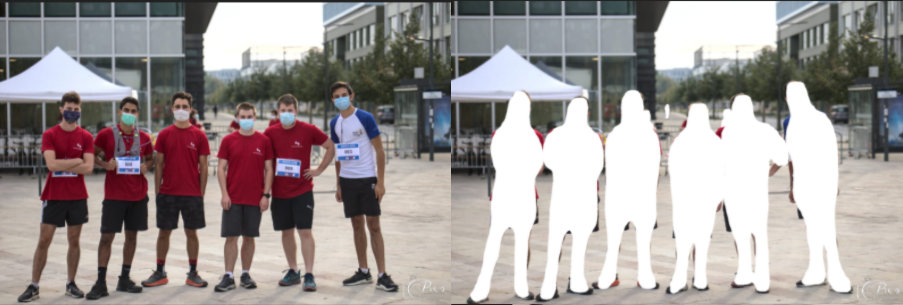
\includegraphics[width=200pts]{images/Mask_R_CNN/resultats_masks_1.png} 
\caption{à gauche : image originelle ; à droite : image dont les personnes ont été enlevées}
\end{figure}

\begin{figure}[!h]
\centering
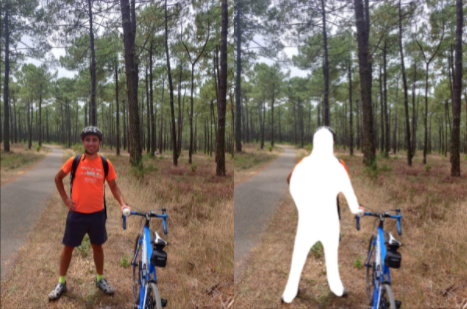
\includegraphics[width=200pts]{images/Mask_R_CNN/resultats_masks_2.png} 
\caption{à gauche : image originelle ; à droite : image dont les personnes ont été enlevées}
\end{figure}